\section{Resultados}\label{sec:resultados}

Todos os valores desta seção foram produzidos pelo software descrito, com os parâmetros da \cref{sec:metodologia}; números citados no texto são gerados a partir dos arquivos de resultado.

\subsection{Validação (E0)}\label{sec:res-validacao}
A \cref{tab:e0} compara as ordens calculadas por Schreier--Sims com os valores da literatura: \gclEzeroAllMatch{} as verificações conferem\ver. A cadeia de estabilizadores de $G$ é obtida em \gclSchreierGTime~ms. A BFS completa do \cube{2} reproduz exatamente a distribuição de distâncias publicada~\cite{oeisA079761,oeisA079762,scherphuis2x2} (\cref{fig:e0}): diâmetro \gclDiamHTM{} em HTM e \gclDiamQTM{} em QTM, com distância média \gclMeanDistHTM{} (HTM) e \gclMeanDistQTM{} (QTM)\ver. As esferas iniciais de $\Cay(G,S)$ no \cube{3} calculadas no E4 também coincidem com as sequências conhecidas~\cite{oeisA080601,oeisA080583}: HTM \gclGhtmSpheres; QTM \gclGqtmSpheres\ver.

\begin{table}[t]
\centering\small
\caption{E0: ordens de grupos calculadas por Schreier--Sims e valores da literatura~\cite{joyner2008,kociembaweb,scherphuis2x2}.}\label{tab:e0}
\begin{tabular}{@{}lrrcr@{}}
\toprule
Grupo & Calculado & Literatura & Confere & ms \\
\midrule
\inputtab{generated/tables/tab_e0_groups.tex}
\bottomrule
\end{tabular}
\end{table}

\begin{figure}[t]
  \centering
  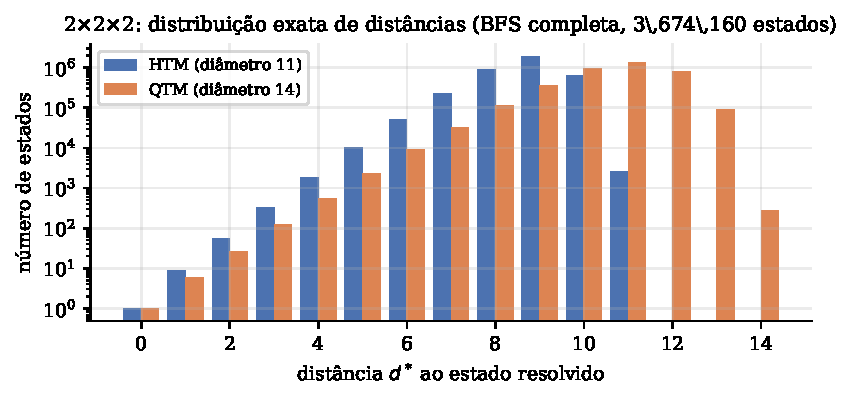
\includegraphics[width=0.86\linewidth]{fig_e0_distribution.pdf}
  \caption{E0: distribuição exata das distâncias no \cube{2} (BFS completa).}
  \label{fig:e0}
\end{figure}

\subsection{Crescimento do espaço de busca (E1)}
A \cref{fig:e1}(a) mostra que $d^*=L$ apenas para embaralhamentos muito curtos: o primeiro caso de $d^*<L$ ocorre em $L=\gclEoneFirstGap$, e para $L\ge14$ a média de $d^*$ é \gclEoneSatMean{}, praticamente a distância média uniforme \gclMeanDistHTM{}. Ou seja, $L$ é um parâmetro do procedimento, não uma medida de dificuldade. Coerentemente, a correlação de postos de Spearman entre esforço da BFS e $d^*$ é \gclEoneRhoD{}, contra \gclEoneRhoL{} com $L$. Em função de $d^*$ (\cref{fig:e1}(b)), o número médio de nós expandidos cresce geometricamente; um ajuste exponencial para $3\le d^*\le9$ dá razão por camada \gclEoneGrowthBFS{} para a BFS e \gclEoneGrowthBi{} para a BFS bidirecional, próximo de $\sqrt{\gclEoneGrowthBFS}\approx\gclEoneGrowthRatio$\proj.

\begin{figure}[t]
  \centering
  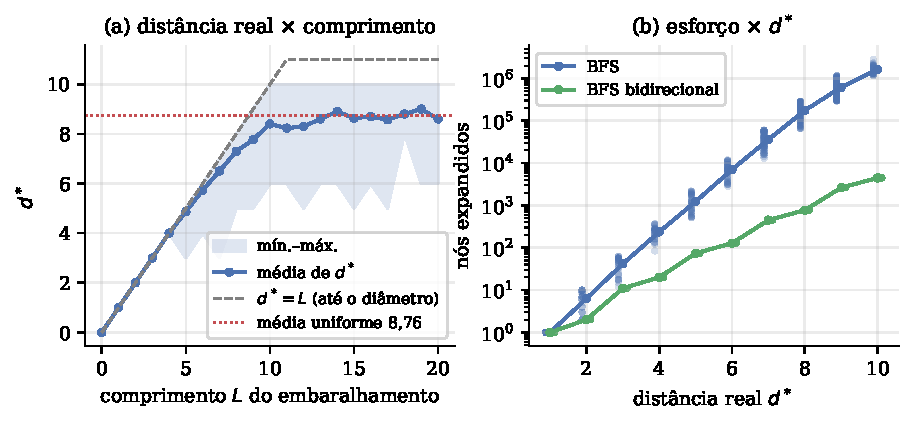
\includegraphics[width=\linewidth]{fig_e1_growth.pdf}
  \caption{E1: (a) distância real $d^*$ versus comprimento do embaralhamento; (b) nós expandidos por instância (pontos) e médias (linhas) em função de $d^*$, escala logarítmica.}
  \label{fig:e1}
\end{figure}

\subsection{Comparação de algoritmos (E2)}
Todas as \gclEtwoRuns{} execuções terminaram com sucesso dentro dos limites e \gclEtwoAllOptimal{} as soluções têm comprimento igual a $d^*$, como garantido pela teoria. A \cref{fig:e2} e a \cref{tab:e2} mostram as diferenças de custo. No caso mais difícil ($d^*=\gclEtwoDmax$), a BFS expande em média \gclEtwoBFSExp{} nós e armazena \gclEtwoBFSPeak{} estados --- praticamente todo o grupo ---, enquanto a BFS bidirecional expande \gclEtwoBFSBiExp{}. A$^*$ com $h_{\max}$ expande \gclEtwoAstarExp{} nós mas armazena \gclEtwoAstarPeak{}; IDA$^*$ expande \gclEtwoIDAstarExp{} nós (mais que A$^*$, por reexpandir nós em iterações sucessivas e não detectar repetidos), armazenando apenas o caminho corrente (\gclEtwoIDAstarPeak{} estados) e sendo o mais rápido (\gclEtwoIDAstarTime~ms de mediana).

\begin{figure}[t]
  \centering
  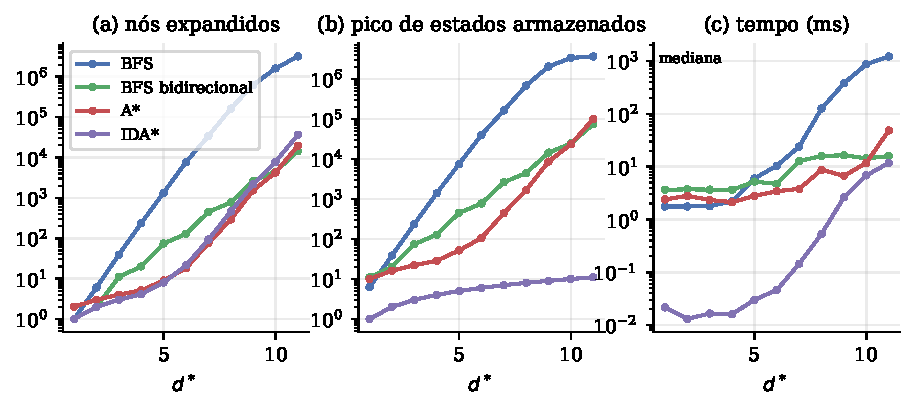
\includegraphics[width=\linewidth]{fig_e2_algorithms.pdf}
  \caption{E2: custo dos algoritmos ótimos em função de $d^*$ (\cube{2}, HTM, \gclEtwoSamples{} estados uniformes por camada).}
  \label{fig:e2}
\end{figure}

\begin{table}[t]
\centering\small
\caption{E2: resumo por algoritmo. Sucesso e otimalidade sobre todas as camadas; expandidos, pico armazenado e tempo (mediana, ms) para $d^*=\gclEtwoDmax$.}\label{tab:e2}
\begin{tabular}{@{}lrrrrr@{}}
\toprule
Algoritmo & Sucesso & Ótimas & Expandidos & Pico armaz. & Tempo \\
\midrule
\inputtab{generated/tables/tab_e2_summary.tex}
\bottomrule
\end{tabular}
\end{table}

\subsection{Heurísticas (E3)}
A \cref{tab:e3} e a \cref{fig:e3} mostram o efeito da heurística. Todas as soluções encontradas são ótimas (\gclEthreeAllOptimal), como esperado de heurísticas admissíveis. A ordem de eficiência acompanha a razão média $h(s_0)/d^*$: $h_0$ (0), $h_{\mathrm{pec}}$ (que nunca excede \gclEthreeMisMax{} no \cube{2}), $h_{\mathrm{ori}}$, $h_{\mathrm{perm}}$, $h_{\max}$ e o oráculo. Em $d^*=\gclEthreeLastD$, IDA$^*$ com $h_{\max}$ expande em média \gclEthreeMaxExp{} nós, \gclEthreeMaxOverPerm{} vezes menos que com $h_{\mathrm{perm}}$ e \gclEthreeMaxOverOri{} vezes menos que com $h_{\mathrm{ori}}$\proj. Com $h_0$, as execuções passam a estourar o limite de \gclEthreeNodeLimit{} nós a partir de $d^*=\gclEthreeZeroFailFrom$; com $h_{\mathrm{pec}}$, a partir de $d^*=\gclEthreeMisFailFrom$. Essas falhas são consequência dos limites declarados, e não de incorreção dos algoritmos. Com o oráculo, IDA$^*$ expande exatamente $d^*$ nós, o mínimo possível.

\begin{table}[t]
\centering\small
\caption{E3: média de nós expandidos por IDA$^*$ (\cube{2}, HTM, \gclEthreeSamples{} estados por camada), fator de ramificação efetivo $b^*$ em $d^*=\gclEthreeLastD$ e razão média $h(s_0)/d^*$. ``---'': todas as execuções atingiram o limite de nós; $^\dagger$: média apenas das execuções bem-sucedidas (algumas atingiram o limite).}\label{tab:e3}
\begin{tabular}{@{}l*{\gclEthreeShowCols}{r}rr@{}}
\toprule
Heurística & \inputtab{generated/tables/tab_e3_heuristics_head.tex} & $b^*$ & $h(s_0)/d^*$ \\
\midrule
\inputtab{generated/tables/tab_e3_heuristics.tex}
\bottomrule
\end{tabular}
\end{table}

\begin{figure}[t]
  \centering
  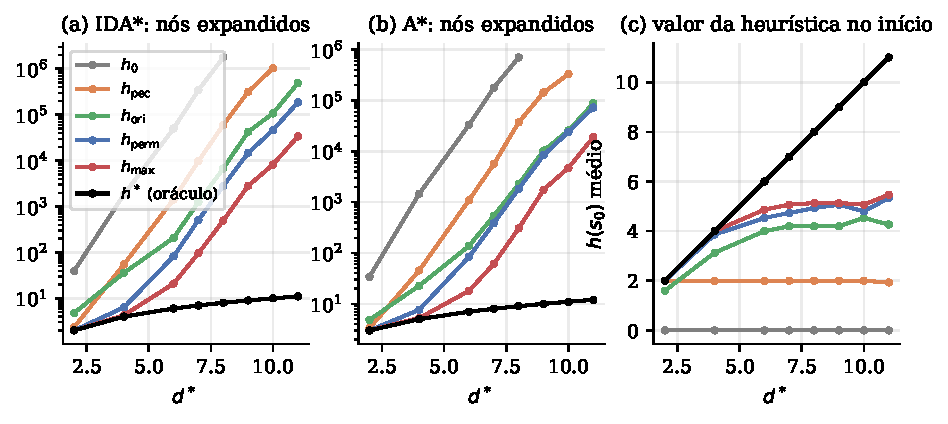
\includegraphics[width=\linewidth]{fig_e3_heuristics.pdf}
  \caption{E3: nós expandidos por IDA$^*$ (a) e A$^*$ (b) para cada heurística, e valor médio da heurística no estado inicial (c).}
  \label{fig:e3}
\end{figure}

\subsection{O \cube{3}: ótimo versus duas fases (E3b)}\label{sec:res-cube3}
Para embaralhamentos de até \gclEthreebLmax{} movimentos, IDA$^*$ com $h_{\mathrm{PDB}}$ terminou em todas as \gclEthreebCount{} instâncias, e em todas elas $d^*$ coincidiu com $L$ (\gclEthreebDstarEqLCount{} de \gclEthreebCount{}). O custo cresce rapidamente: em $L=\gclEthreebLmax$, a média foi de \gclEthreebPdbExpLast{} nós expandidos e a mediana de \gclEthreebPdbTimeLast~s (\cref{tab:e3b,fig:e3b}). A heurística $h_{\mathrm{pec}}$, executada até $L=7$, expande de 50 a 90 vezes mais nós que $h_{\mathrm{PDB}}$ em $L\in\{6,7\}$ (\cref{tab:e3b}). O método de duas fases (200~ms) encontrou a solução ótima em \gclEthreebTPOptimalPct\% das instâncias curtas, com excesso máximo de \gclEthreebTPExcessMax{} movimentos.

Em \gclTPUniformN{} estados uniformes de $G$, a \emph{primeira} solução de duas fases tem em média \gclTPFirstMean{} movimentos (de \gclTPFirstMin{} a \gclTPFirstMax; mediana de tempo \gclTPFirstTimeMed~ms); continuando a busca até obter $\le20$ ou esgotar 1~s, a média cai para \gclTPTargetMean{} (máximo \gclTPTargetMax; \gclTPTargetLe\% com $\le20$ movimentos; mediana \gclTPTargetTimeMed~ms). Nenhum desses números contradiz o diâmetro 20 de $G$~\cite{rokicki2014}: as soluções de duas fases são válidas, mas não mínimas, e o limite de tempo pode interromper a busca antes de alcançar 20.

\begin{table}[t]
\centering\small
\caption{E3b: embaralhamentos do \cube{3} (\gclEthreebSamples{} por $L$). $d^*$ é o comprimento encontrado por IDA$^*$ com $h_{\mathrm{PDB}}$ (ótimo). Tempos em ms (mediana). n.e.: não executado ($h_{\mathrm{pec}}$ apenas para $L\le7$).}\label{tab:e3b}
\begin{tabular}{@{}rrrrrrr@{}}
\toprule
& & \multicolumn{2}{c}{IDA$^*$ $h_{\mathrm{PDB}}$} & \multicolumn{2}{c}{IDA$^*$ $h_{\mathrm{pec}}$} & Duas fases \\
\cmidrule(lr){3-4}\cmidrule(lr){5-6}\cmidrule(l){7-7}
$L$ & $d^*$ & expandidos & tempo & expandidos & tempo & comprimento \\
\midrule
\inputtab{generated/tables/tab_e3b.tex}
\bottomrule
\end{tabular}
\end{table}

\begin{figure}[t]
  \centering
  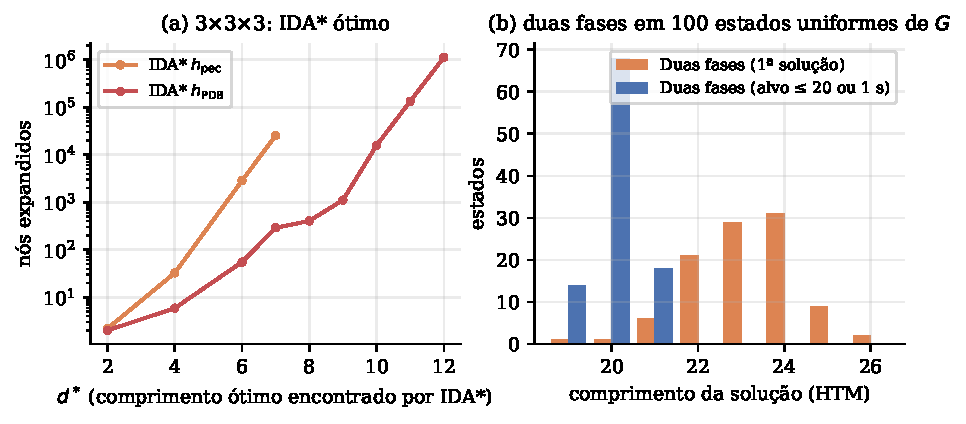
\includegraphics[width=\linewidth]{fig_e3b_cube3.pdf}
  \caption{E3b: (a) nós expandidos por IDA$^*$ no \cube{3}; (b) comprimentos das soluções de duas fases em estados uniformes de $G$.}
  \label{fig:e3b}
\end{figure}

\subsection{Estrutura dos grafos de Cayley (E4)}
A \cref{tab:e4} resume a estrutura dos \gclEfourSets{} grafos. Algumas observações\proj:
\begin{itemize}[nosep]
\item \emph{Geradores de meia-volta criam triângulos.} Incluir $X^2$ junto com $X$ produz a relação $X\,X\,X^2=e$ e cintura 3; com apenas quartos de volta, a cintura é 4 ($X^4=e$, ou um par de geradores que comutam, como $\mv{U2}\,\mv{D2}\,\mv{U2}\,\mv{D2}$ no grupo dos quadrados).
\item \emph{Grupos diédricos.} $\langle\mv{R2},\mv{U2}\rangle$ tem ordem 12 no \cube{3} (e 6 no \cube{2}): o grafo de Cayley é um ciclo de 12 vértices e a menor relação é $(\mv{U2}\,\mv{R2})^6$.
\item \emph{Mesma ordem, diâmetros diferentes.} No \cube{2}, $\langle\mv R,\mv U\rangle$ tem 29\,160 elementos e diâmetro \gclEfourRUTwoDiamQ{} em QTM, mas \gclEfourRUTwoDiamH{} quando se admitem meias-voltas. O subgrupo $\langle\mv R,\mv{U2}\rangle$ do \cube{3}, com apenas 14\,400 elementos, tem diâmetro \gclEfourRUtwoThreeDiam{}, maior que o de $G_2$: geradores ``pobres'' produzem grafos finos e longos.
\item \emph{Grupo dos quadrados.} $\langle\mv{U2},\dots,\mv{B2}\rangle$ ($663\,552$ elementos) foi enumerado completamente: diâmetro \gclEfourSqDiam{} e distância média \gclEfourSqMean{}; seu conjunto gerador é preservado pelas 48 simetrias do cubo.
\item \emph{Crescimento.} Nos grupos grandes, as esferas crescem geometricamente até a ``metade'' do grafo e depois decrescem (\cref{fig:e4}); a cota $|S|(|S|-1)^{r-1}$ só é atingida enquanto não há relações curtas.
\end{itemize}

\begin{table}[t]
\centering\footnotesize\setlength{\tabcolsep}{3.2pt}
\caption{E4: estrutura de $\Cay(\langle S\rangle,S\cup S^{-1})$. Grau $=|S\cup S^{-1}|$; ``$r\le k$'': bola exata até o raio $k$ (grafo não enumerado); diâmetro e distância média só quando completo; Sim.: simetrias do cubo (de 48) que preservam $S$.}\label{tab:e4}
\begin{tabular}{@{}lrrcrrrr@{}}
\toprule
Conjunto & $|\langle S\rangle|$ & Grau & Completo & Diâm. & Dist. média & Cintura & Sim. \\
\midrule
\inputtab{generated/tables/tab_e4.tex}
\bottomrule
\end{tabular}
\end{table}

\begin{figure}[t]
  \centering
  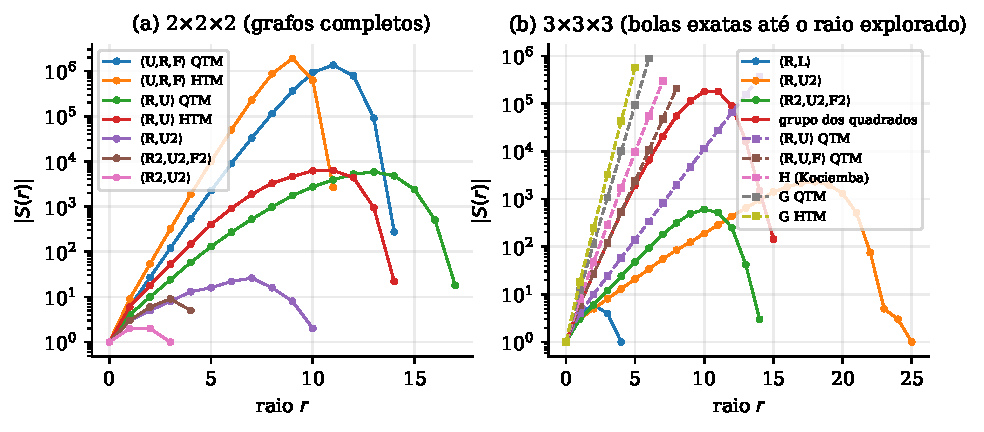
\includegraphics[width=\linewidth]{fig_e4_spheres.pdf}
  \caption{E4: tamanhos das esferas $|S(r)|$ (linhas cheias: grafos completos; tracejadas: bolas parciais, exatas até o raio mostrado).}
  \label{fig:e4}
\end{figure}
